\chapter{Damage detection and predicting fire behavior and condition}
	\label{cha:methodology}
	
	Procedures for predicting the spread of fire include:
	
	\begin{itemize}
		\item Evaluation of installation fuel, fuel moisture, wind speed, surface slope.
		\item Estimation of fire spread speed and intensity.
		\item Methods for interpreting the speed and intensity of a fire to obtain the distance, perimeter, area, and conditions under which stains and crowns occur. An important feature is the determination of the probable time of fire growth on a map over a period of time.
	\end{itemize}

	The diagram below shows the flow in information system to implement the fire behavior prediction (Choi et al. 2020):
	
	\begin{figure}[H]
		\centering
		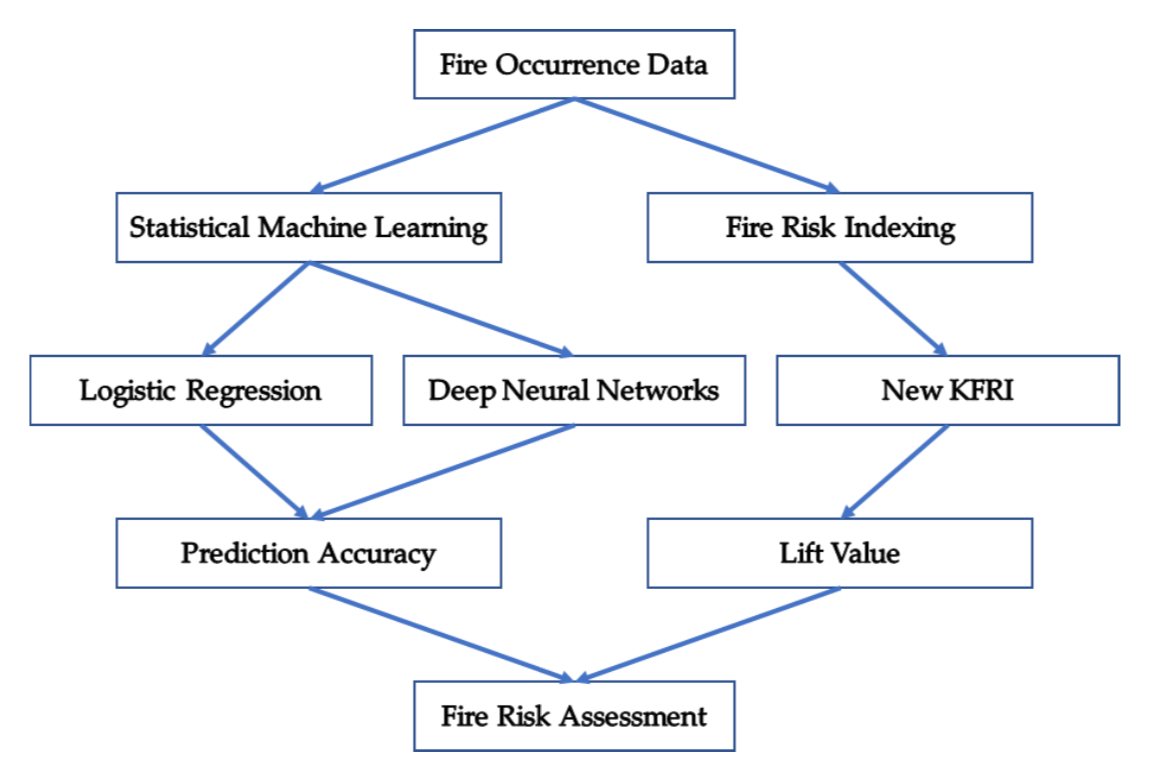
\includegraphics[width=0.9\linewidth]{images/fire_assesment_procedure.png}
		\caption{Procedure for fire risk assessment}
		\label{fig:fire_assesment_procedurel}
	\end{figure}
	
\section{Wildfire damage detection methodology using passive remote sensing data}

	To determine the damage from a forest fire, a relatively normalized installation index can be used, which allows to determine the intensity ranges of the damaged forest.
	
	The application of the forest fire damage detection methodology was performed using the Sentinel-2 group satellite Sentinel-2A with passive remote sensing sensors, which was launched into orbit in 2015.
	
	In order to determine whether the data provided is suitable for solving GIS tasks, a survey was conducted in 2017. Determination of fire damage in Portugal. Sentinel-2A data used for the study are from 04/06/2017 to 04/07/2017.
	
	Forest fire damage was used in 2017. in central Portugal, in the Pedrógão Grand region, Sentinel-2A satellite data before and after the fire. The corresponding indices (before and after the fire) were calculated using raster algebra (pixel composition, subtraction, multiplication and division of different wavebands) and the results were compared with each other.
	
	Before indexing, the initial data must be prepared by performing the appropriate image processing.
	
	Sentinel-2A data has cloud information, so using SNAP software we can use this information for a cloud mask creation.
	
	\begin{lstlisting}
	if (
		scl_cloud_medium_proba + 
		scl_cloud_high_proba +                                                			      
		scl_thin_cirrus
	) < 255 then 0 else 1
	\end{lstlisting}
	
	where $scl\_cloud\_medium\_proba$, $scl\_cloud\_high\_proba$, and $scl\_thin\_cirrus$ cloud data, which distinguishes clouds from the original data.
	
	This filter is used to perform raster algebra in SNAP software for removing clouds. After performing raster algebra and applying the above cloud filter, an additional band in the raster data set is obtained, which is required in the following data processing steps.
	
	A normalized burn index is most commonly used to isolate vegetation damaged during a fire. This index is calculated according to the following formula (Parks et al., 2014):
	
	\begin{equation}
	NBR=\dfrac{NIR - SWIR}{NIR + SWIR}
	\end{equation}
	
	where $NIR$ - infrared wavelenght band, $SWIR$ - shortwave infrared color band.
	
	The higher the normalized implementation index, the vegetation in the study area is the least damaged and vice versa, the lower the index, the more damaged the vegetation (Coppoletta, M et al., 2016) (fig. \ref{fig:nbr_index}).
	
	\begin{figure}[H]
		\centering
		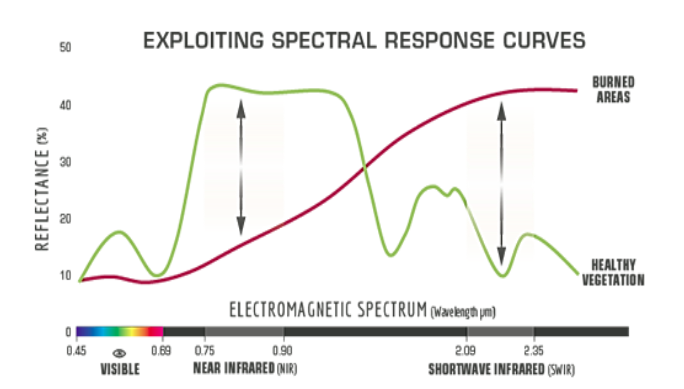
\includegraphics[width=0.9\linewidth]{images/nbr_index.png}
		\caption{The NBR index was determined in the SNAP software}
		\label{fig:nbr_index}
	\end{figure}

	To refine the results, a normalized water index is determined that separates water from the forest vegetation. Calculation formula (Du et al., 2016):
	
	\begin{equation}
	NDWI = \dfrac{Green - NIR}{Green + NIR}
	\end{equation}
	
	where $NIR$ - inrared color band and $Green$ - green color band
	
	After performing raster algebra, the hydrological layer and raster data are separated.
	
	To determine the final forest damage, a relative deployment index is calculated, which determines the ratio of the deployment index before and after the fire (Parks, S, et al. 2014):
	
	\begin{equation}
	\label{eq:dnbr}
	dNBR = \dfrac{NBR_{pre_fire} - NBR_{post_fire}}{NBR_{pre-fire} + 1.001}
	\end{equation}
	
	where $NBR_{pre_fire}$ - normalized installation index before fire, $NBR_{post_fire}$ - normalized installation index after fire.
	
	The intervals of the $dNBR$ index allow to determine the extent of forest damage (tab. \ref{tab:nbi-res}). These intervals are used for the final visualization of the processed data and presentation of the results.
	
	
	{\setlength{\extrarowheight}{15pt}%
	\begin{table}[H]
		\begin{center}
			\caption{$dNBR$ index interval burn intervals (Tonbul, H et al., 2016)}
			\label{tab:nbi-res}
			\begin{tabularx}{\textwidth}{|X|X|}
				\hline
				\textbf{dNBR} & \textbf{Burn severity}\\
				\hline
				< -0.25 & Enhanced regrowth after fire, high \\
				\hline
				from -0.25 to -0.1 & Enhanced regrowth after fire, low  \\
				\hline
				from -0.1 to 0.1 & Unburned \\
				\hline
				from 0.1 to 0.27 & Low severity \\
				\hline
				from 0.27 to 0.44 & Moderate low severity \\
				\hline
				from 0.44 to 0.66 & Moderate high severity \\
				\hline
				> 0.66 & High severity \\
				\hline
			\end{tabularx}
		\end{center}
	\end{table}

	The calculation of $dNBR$ is performed by applying normalized water index and cloud cover filters and applying formula \ref{eq:dnbr}. After calculating the $dNBR$, a raster data set was obtained, the pixel values of which determine the degree of forest burn (fig. \ref{fig:dnbr}).
	
	\begin{figure}[H]
		\centering
		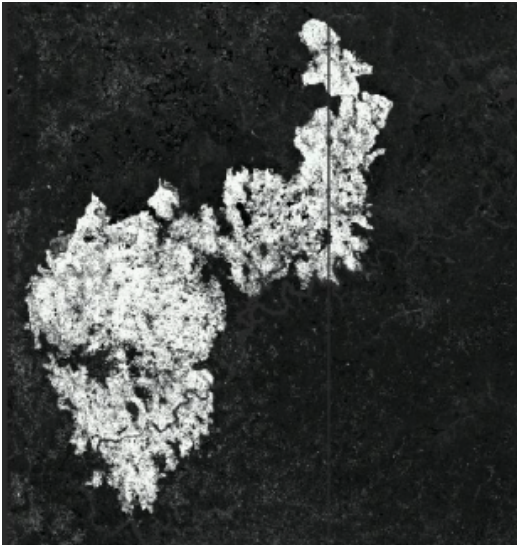
\includegraphics[width=0.9\linewidth]{images/dnbr.png}
		\caption{Calculated $dNBR$ index as thematic map in \textit{QGIS} application}
		\label{fig:dnbr}
	\end{figure}

	In order to quantify the area in each burn severity class, the statistics of the raster must be calculated. A transformation of the raster, so that all pixels are assigned one value for each burn severity class is necessary. in addition to this we excluded regrowth in the classification and applied the full table of classification (Table \ref{tab:nbi-res}).
	
	By using raster calculator every value in raster is multiplied by 1000 so it would be possible to apply classifier that will extract area for concrete burn area:
	
	\begin{figure}[H]
		\centering
		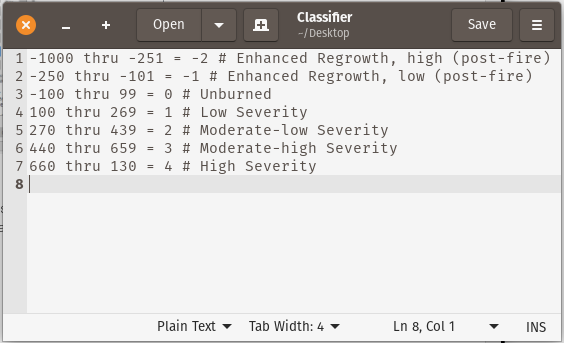
\includegraphics[width=0.9\linewidth]{images/rules_classifier.png}
		\caption{Rules for which pixels are attributed to which class}
		\label{fig:dnbr}
	\end{figure}

	By using \textit{QGIS r.report} processing toolbox it is possible to get report with calculated area of fire severity:
	
	{\setlength{\extrarowheight}{15pt}%
	\begin{table}[H]
		\begin{center}
			\caption{Report of rater statistic by severity level}
			\label{tab:nbi-res}
			\begin{tabularx}{\textwidth}{|X|X|}
				\hline
				\textbf{Severity level} & \textbf{Area, ha}\\
				\hline
				-2 & 6.787 \\
				\hline
				-1 & 350.308  \\
				\hline
				0 & 8553.005 \\
				\hline
				1 & 11969.245 \\
				\hline
				2 & 12354.006 \\
				\hline
				3 & 11388.385 \\
				\hline
				4 & 11010.700 \\
				\hline
			\end{tabularx}
		\end{center}
	\end{table}

	
	
	
	
	
